% mystylefile.pandoc
\usepackage[Lenny]{fncychap}
\usepackage{fancyhdr}
\pagestyle{fancy}
\fancyhf{}
\fancyhead[LE,RO]{\thepage}
\fancyhead[RE]{\leftmark}
\fancyhead[LO]{\rightmark}
\usepackage{tcolorbox}
\newtcolorbox{myquote}{colback=red!5!white, colframe=red!75!black}
\newtcolorbox{myverbatim}{colback=green!5!white, colframe=green!75!black}
% redefine the 'quote' environment to use this 'myquote' environment
\renewenvironment{quote}{\begin{myquote}}{\end{myquote}}

\usepackage{etoolbox}
\makeatletter
\patchcmd{\@verbatim}
  {\verbatim@font}
  {\verbatim@font\small}
  {}{}
\makeatother

\chapterfont{\clearpage}
\renewenvironment{Shaded}{\begin{snugshade}\small}{\end{snugshade}}

\usepackage{caption}
\captionsetup{labelformat=empty, font={sl}}

% for background image
\usepackage[pages=some]{background}
\backgroundsetup{
scale=1,
color=black,
opacity=0.15,
angle=0,
contents={%
  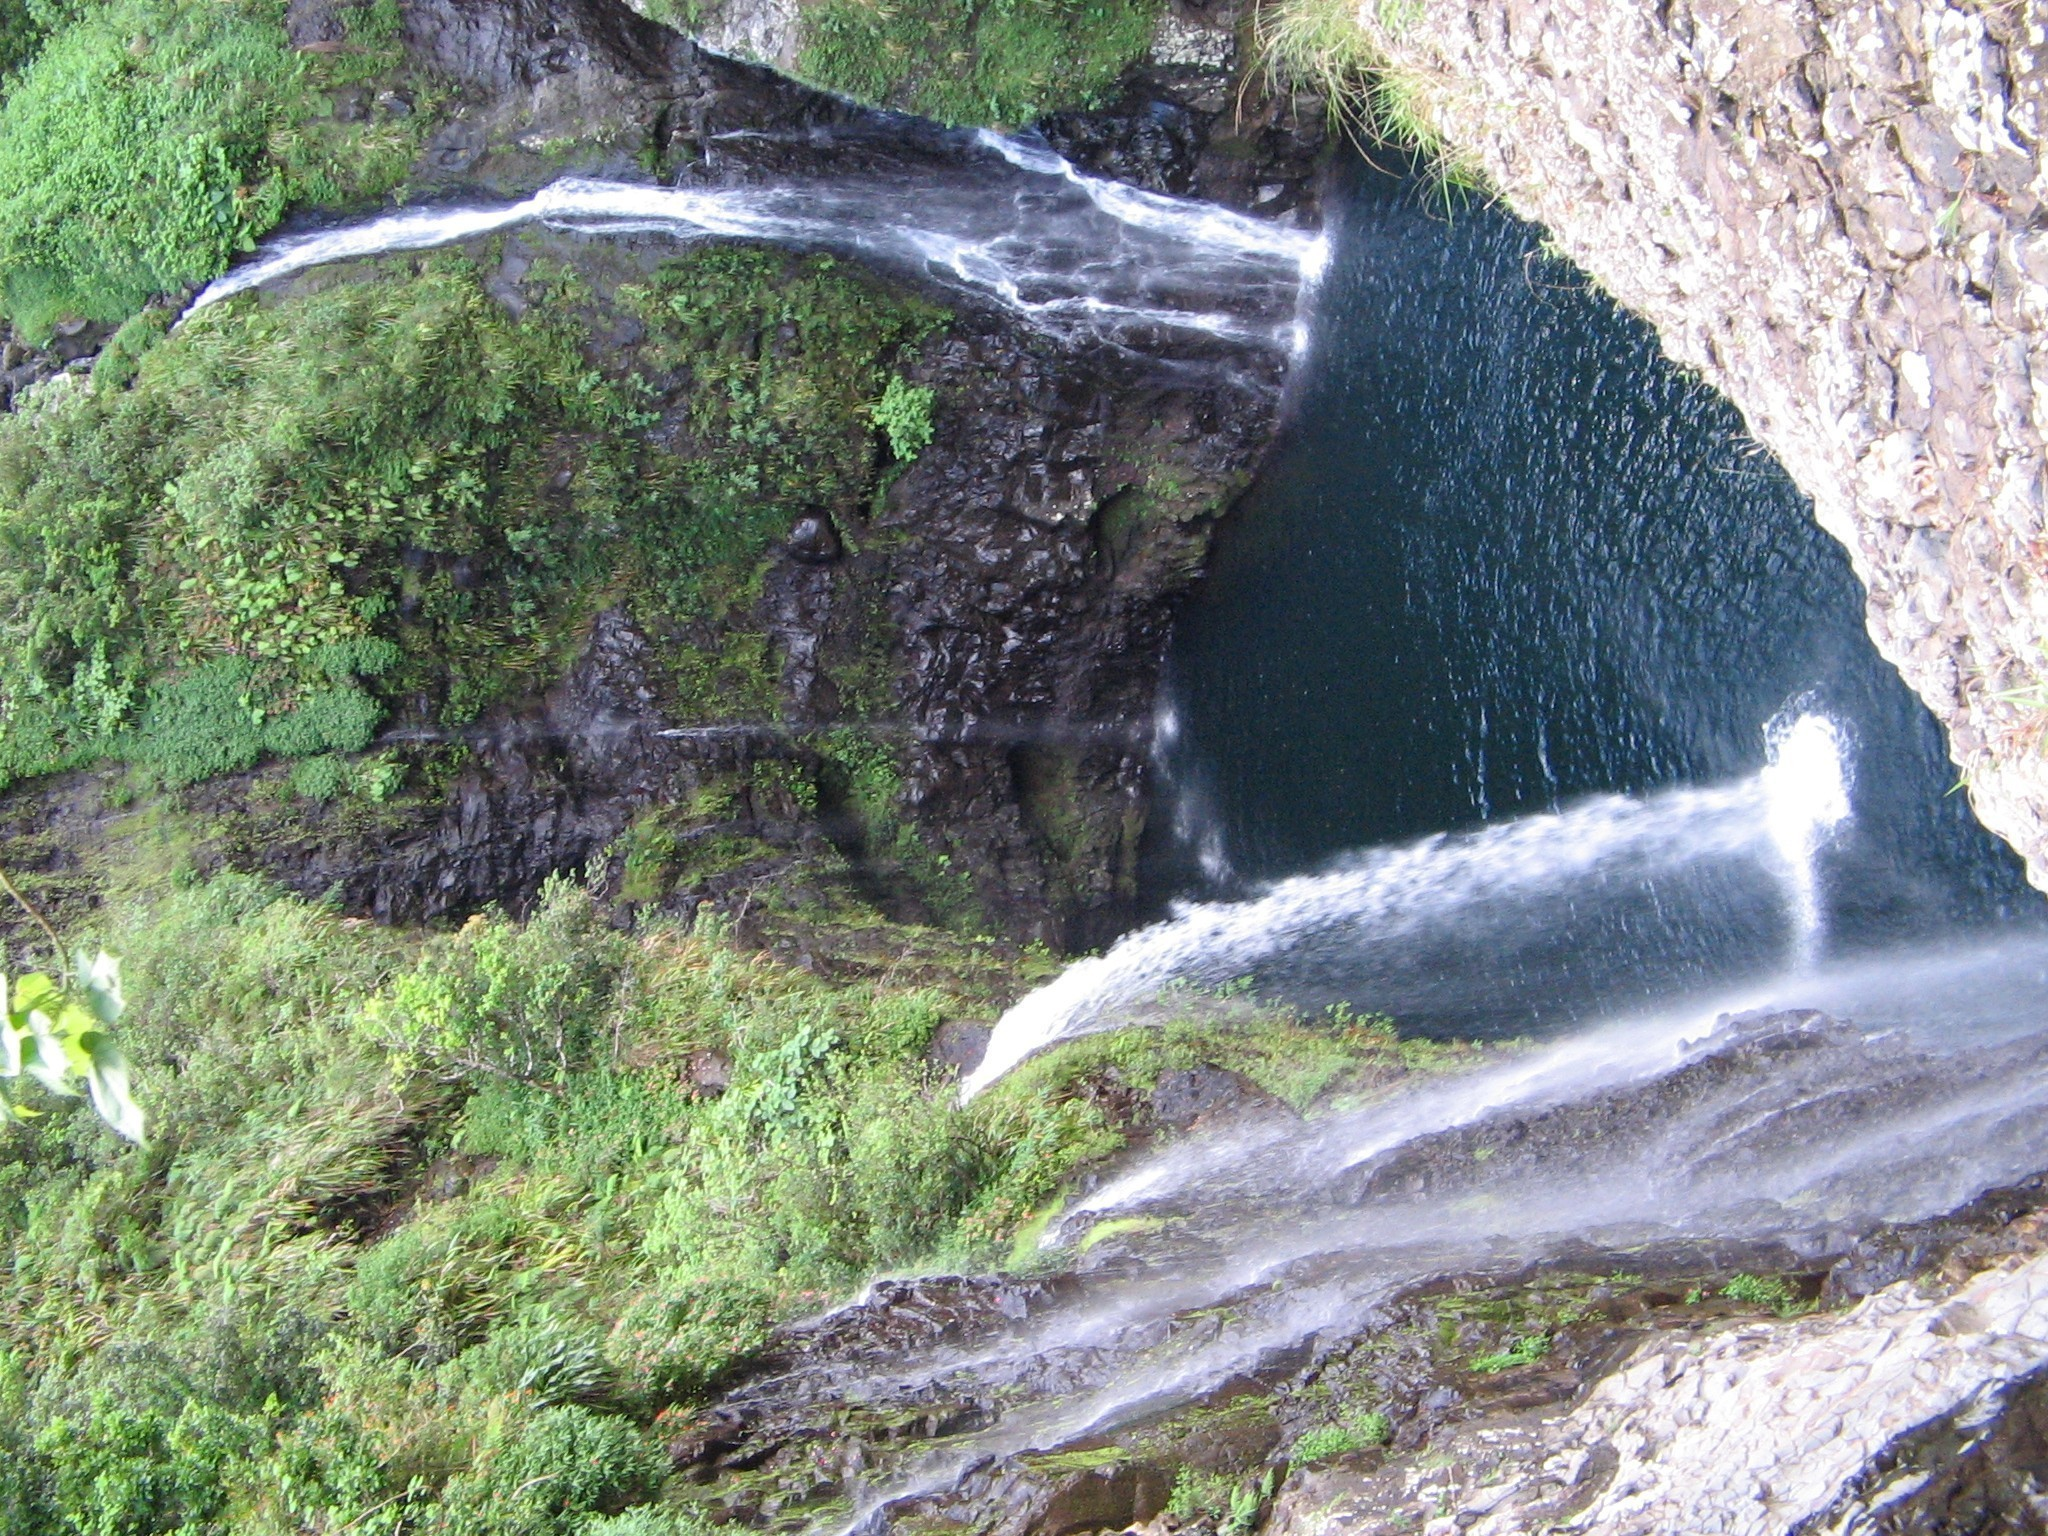
\includegraphics[width=\paperwidth,height=\paperheight,angle=-90]{pics/takamaka.jpg}
  }%
}

\BgThispage
%% temporary titles
% command to provide stretchy vertical space in proportion
\newcommand\nbvspace[1][3]{\vspace*{\stretch{#1}}}
% allow some slack to avoid under/overfull boxes
\newcommand\nbstretchyspace{\spaceskip0.5em plus 0.25em minus 0.25em}
% To improve spacing on titlepages
\newcommand{\nbtitlestretch}{\spaceskip0.6em}
\pagestyle{empty}
\begin{center}
\bfseries
\nbvspace[1]
\Huge
{\nbtitlestretch\huge
PROGRAMMING HOTMOKA}

\nbvspace[1]
\normalsize

LEARN HOW TO PROGRAM HOTMOKA NODES\\
WITH SMART CONTRACTS IN PURE JAVA
\nbvspace[1]\\
\Large FAUSTO SPOTO\\[0.5em]
\footnotesize ASSOCIATE PROFESSOR\\
DEPARTMENT OF COMPUTER SCIENCE\\
UNIVERSITY OF VERONA, ITALY

\nbvspace[2]


\includegraphics[width=1in]{./pics/logo_hotmoka_minimal.png}
\nbvspace[2]
\normalsize

\nbvspace[1]

\includegraphics[width=0.5in]{./pics/CC_license.png}\\
\small
This work is licensed under a Creative Commons Attribution 4.0 International License

\end{center}

\newpage

\nbvspace[2]
The latest version of this document is available for free in PDF, ePub and MOBI format, at \url{https://github.com/Hotmoka/hotmoka/releases}.
